% Documento de diseño (GDD) — Barrel Ascent
% Compilar: tectonic GDD_BarrelAscent.tex
\documentclass[11pt,letterpaper]{article}
\usepackage{fontspec}
\usepackage[spanish,es-noshorthands]{babel}
\usepackage[margin=2cm,top=1.8cm,bottom=1.8cm]{geometry}
\usepackage{graphicx}
\usepackage{booktabs}
\usepackage{tabularx}
\usepackage{xcolor}
\usepackage{enumitem}
\usepackage{tikz}
\usetikzlibrary{arrows.meta,positioning}
\usepackage{titlesec}
\usepackage{fancyhdr}
\usepackage{caption}
\usepackage{float}
\usepackage[hidelinks]{hyperref}

% ---- Datos del alumno (editar aquí) ----
\newcommand{\alumno}{Ashley Peña Nolasco}
\newcommand{\matricula}{178226}
% ----------------------------------------

\definecolor{acento}{HTML}{875333}
\definecolor{oscuro}{HTML}{182B38}
\titleformat{\section}{\large\bfseries\color{oscuro}}{\thesection.}{0.5em}{}
\titlespacing*{\section}{0pt}{8pt}{3pt}
\setlist{nosep,leftmargin=1.2em}
\setlength{\parskip}{3pt}
\setlength{\parindent}{0pt}
\pagestyle{fancy}\fancyhf{}
\lhead{\small Barrel Ascent --- Documento de diseño}
\rhead{\small Laboratorio de Videojuegos}
\cfoot{\small \thepage}
\renewcommand{\headrulewidth}{0.4pt}

\begin{document}

\begin{center}
{\LARGE\bfseries\color{oscuro} Barrel Ascent}\\[2pt]
{\large Documento de diseño del videojuego (GDD)}\\[6pt]
\begin{tabular}{ll}
\textbf{Alumno:} \alumno & \textbf{ID:} \matricula\\
\textbf{Curso:} Laboratorio de Videojuegos & \textbf{Modalidad:} Crédito por examen\\
\textbf{Tecnología:} Unity 6 (6000.4) con C\# & \textbf{Plataforma:} macOS (escritorio)
\end{tabular}
\end{center}

\section{Concepto}
\emph{Barrel Ascent} es un juego de plataformas 2D en pixel art de una sola partida corta
(3--5 minutos). El jugador controla a una técnica de mantenimiento que debe subir por el
interior de una fábrica vertical, piso a piso, usando escaleras y saltos, mientras una línea de
producción descontrolada lanza barriles que ruedan por las vigas y caen en zigzag hacia abajo.
Hay que esquivarlos o saltar sobre ellos, recoger piezas de repuesto y llegar a la baliza de la cima.

\textbf{Frase de venta:} \emph{``Sube, esquiva y pisa: la fábrica entera rueda contra ti.''}

\section{Historia y premisa}
Una antigua fábrica de barriles se reactivó sola durante la noche: la línea automática de la azotea
expulsa barriles sin control y los deja caer por todos los pisos. La técnica de turno es la única
dentro del edificio y el único modo de detener la línea es activar la \textbf{baliza de emergencia}
de la cima. El recorrido atraviesa tres zonas: la \emph{Base industrial}, la sala de
\emph{Maquinaria} y \emph{La cima}. Por el camino recoge engranajes, componentes y cápsulas que
servirán para reparar la máquina.

La premisa justifica el diseño: el ascenso explica la estructura vertical del nivel; la línea
descontrolada explica que los barriles aparezcan siempre desde arriba y cada vez más rápido; y la
baliza ofrece un objetivo único y visible desde lejos.

\section{Tipo de videojuego y referentes}
\textbf{Género:} plataformas de acción 2D de pantalla vertical (\emph{arcade platformer}),
para un jugador. Pertenece a la tradición de los plataformas arcade de principios de los ochenta
(por ejemplo, \emph{Donkey Kong}, Nintendo, 1981), que definieron el esquema de vigas,
escaleras y obstáculos rodantes que bajan mientras el jugador sube. \emph{Barrel Ascent} toma
de ese género la mecánica base (subir, esquivar, saltar) y la adapta con elementos modernos:
cámara con desplazamiento vertical en lugar de pantalla fija, zonas con dificultad progresiva,
pisotón con rebote como forma de defensa y \emph{coyote time} y \emph{jump buffer} para que el salto
se sienta justo. Personajes, arte, nivel y sonidos son propios del proyecto.

\section{Usuario objetivo}
Jugadores casuales de 10 años en adelante y aficionados a los juegos retro que buscan partidas cortas
con reglas que se entienden en segundos. No requiere experiencia previa: solo teclado, controles
mostrados en el menú y una curva de dificultad que empieza lenta. La clasificación orientativa es
\emph{para todos} (sin violencia gráfica: los barriles se rompen en astillas).

\section{Reglas}
\begin{tabularx}{\linewidth}{@{}lX@{}}
\toprule
\textbf{Elemento} & \textbf{Regla} \\ \midrule
Vidas & Se empieza con 3 vidas (corazones en el HUD). \\
Golpe de barril & Contacto lateral: $-1$ vida, retroceso y 1,5\,s de invulnerabilidad (parpadeo). \\
Caída del nivel & Caer por debajo del suelo: $-1$ vida y reaparición en el punto seguro de la zona más alta alcanzada. \\
Pisotón & Caer sobre un barril lo destruye: $+50$ puntos y rebote hacia arriba, sin daño. \\
Coleccionable & 10 piezas en el nivel; cada una vale $+100$ y solo se recoge una vez. \\
Zona superada & Entrar por primera vez en la zona siguiente: $+250$ (no se repite). \\
Meta & Tocar la baliza: $+250$ (zona 3) $+1000$ y \textbf{victoria}. \\
Derrota & Perder la tercera vida: \textbf{Game Over}. \\
Puntuación & Solo cambia durante el juego activo; máximo sin barriles: 2750 puntos. \\
\bottomrule
\end{tabularx}

\section{Mecánicas}
\begin{enumerate}[label=\textbf{M\arabic*.}]
\item \textbf{Movimiento y salto.} Desplazamiento lateral a 5\,u/s y salto de unos 1,7 tiles; un solo
salto por contacto con el suelo (sin doble salto), con tolerancias de 0,08\,s tras dejar el borde
(\emph{coyote time}) y 0,1\,s antes de aterrizar (\emph{jump buffer}).
\item \textbf{Escalar.} Dentro de una escalera, arriba/abajo sube o baja sin gravedad; no se puede saltar
ni moverse de lado mientras se escala. Al terminar, el personaje queda de pie sobre la plataforma.
\item \textbf{Evasión de barriles.} Los barriles ruedan por cada viga, caen por el extremo abierto e
invierten el sentido en el piso inferior. El jugador los salta, espera en una escalera o los rodea.
\item \textbf{Pisotón.} Aterrizar encima de un barril lo destruye y da un rebote que permite encadenar
movimientos: convierte el peligro en recompensa.
\item \textbf{Recolección.} Piezas flotantes colocadas fuera de la ruta más corta para premiar el riesgo.
\end{enumerate}

\section{Controles}
\begin{tabularx}{\linewidth}{@{}lX@{}}
\toprule
\textbf{Acción} & \textbf{Teclado} \\ \midrule
Mover & A / D o flechas izquierda/derecha \\
Subir / bajar escalera & W / S o flechas arriba/abajo \\
Saltar & Espacio \\
Pausa / reanudar & Esc (o botón de pausa del HUD) \\
Reiniciar & R (solo tras victoria o derrota) \\
Menús & Ratón, o flechas + Enter/Espacio \\
\bottomrule
\end{tabularx}

\section{Escenas y flujo de juego}
\vspace{-2pt}
El juego tiene dos escenas: \textbf{MainMenu} (título, botones \emph{Jugar} y \emph{Salir}, controles) y
\textbf{GameLevel} (el nivel completo con HUD). Dentro de \emph{GameLevel}, los estados de la partida se
muestran con paneles superpuestos. La Figura~\ref{fig:flujo} resume el flujo.

\begin{figure}[H]
\centering\vspace{-4pt}
\begin{tikzpicture}[>=Stealth,
  st/.style={draw=oscuro, fill=oscuro!8, rounded corners, minimum width=22mm, minimum height=6mm, font=\small},
  lb/.style={font=\scriptsize}]
\node[st] (menu) at (0,0) {Menú principal};
\node[st] (play) at (4.6,0) {Juego activo};
\node[st] (pause) at (9.6,0) {Pausa};
\node[st] (lost) at (2.2,-1.45) {Game Over};
\node[st] (won) at (7.0,-1.45) {Victoria};
\draw[->] (menu) -- node[above,lb]{Jugar} (play);
\draw[->] (play.15) -- node[above,lb]{Esc (ida) / Reanudar o Esc (vuelta)} (pause.165);
\draw[->] (pause.195) --  (play.345);
\draw[->] (play.250) -- node[left,lb,pos=0.7]{0 vidas} (lost.north);
\draw[->] (play.290) -- node[right,lb,pos=0.7]{toca la baliza} (won.north);
\draw[->,dashed] (lost.west) -| node[pos=0.7,left,lb]{Menú} (menu.south);
\draw[->,dashed] (won.east) -| node[pos=0.7,right,lb]{Menú} (pause.south);
\draw[->,dashed] (lost.east) -- node[above,lb]{Reiniciar (R)} (won.west);
\end{tikzpicture}
\caption{Flujo de escenas y estados de la partida. Las líneas punteadas son opciones de los paneles:
desde Game Over y Victoria se reinicia (botón o tecla R) o se vuelve al menú; desde Pausa también.}\label{fig:flujo}
\end{figure}

\begin{figure}[h]
\centering
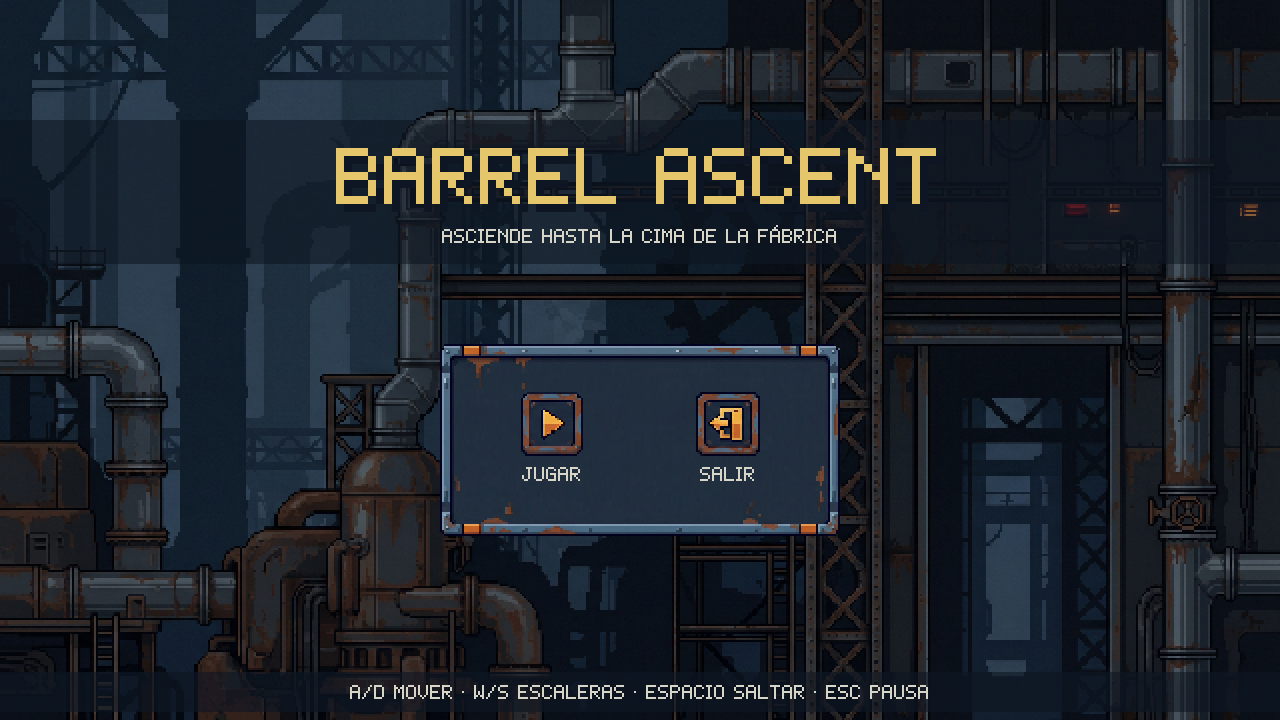
\includegraphics[width=0.48\linewidth]{figs/UI_MainMenu.png}\hfill
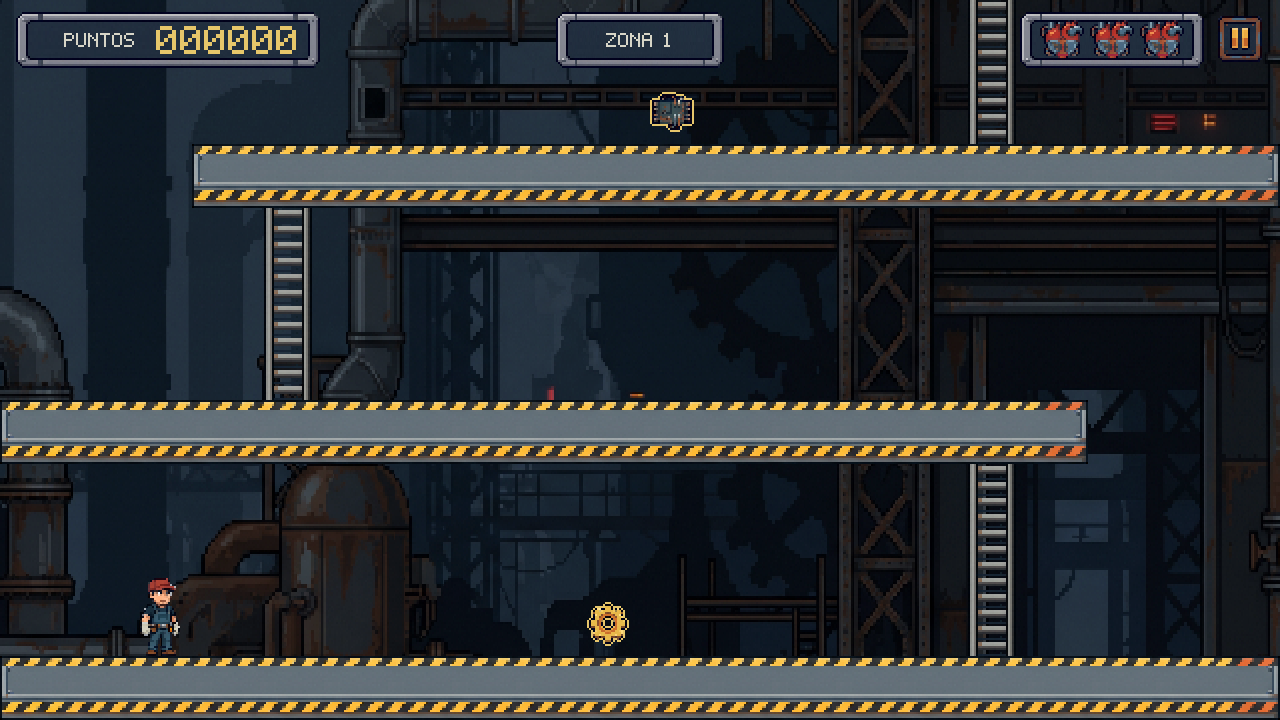
\includegraphics[width=0.48\linewidth]{figs/UI_HUD.png}
\caption{Menú principal (izq.) y juego activo con HUD: puntuación, zona actual, vidas y pausa (der.).}
\end{figure}

\section{Nivel: escena principal}
\noindent\begin{minipage}[t]{0.74\linewidth}
\vspace{0pt}
Un único nivel vertical de $20\times46$ tiles (32\,px), con 12 escaleras, 10 coleccionables y la meta
arriba (Fig.~\ref{fig:nivel}). La cámara muestra $20\times11{,}25$ tiles y sigue al jugador solo en
vertical. Cada zona tiene un fondo propio y su propio generador de barriles, que solo está activo
mientras el jugador se encuentra en ella.

\smallskip
\begin{tabularx}{\linewidth}{@{}lX@{}}
\toprule
\textbf{Zona} & \textbf{Diseño y dificultad} \\ \midrule
1. Base industrial & Vigas anchas con un extremo abierto alterno; una escalera por piso. Barriles a 2\,u/s cada 4\,s. \\
2. Maquinaria & Escalón de un tile, hueco de dos tiles, dos escaleras por piso. Barriles a 2,75\,u/s cada 3\,s. \\
3. La cima & Vigas estrechas con huecos de dos tiles; la baliza en el último piso. Barriles a 3,5\,u/s cada 2\,s. \\
\bottomrule
\end{tabularx}

\smallskip
Los extremos abiertos alternos hacen que cada barril baje en zigzag, cruzando la ruta del jugador
en cada piso. Hay como máximo 6 barriles vivos por zona. Si el jugador cae, reaparece en el punto
seguro de la zona más alta que haya alcanzado (inicio del nivel o primera escalera de las zonas 2 y 3),
así que el progreso vertical nunca se pierde por completo.
\end{minipage}\hfill
\begin{minipage}[t]{0.23\linewidth}
\vspace{0pt}\centering
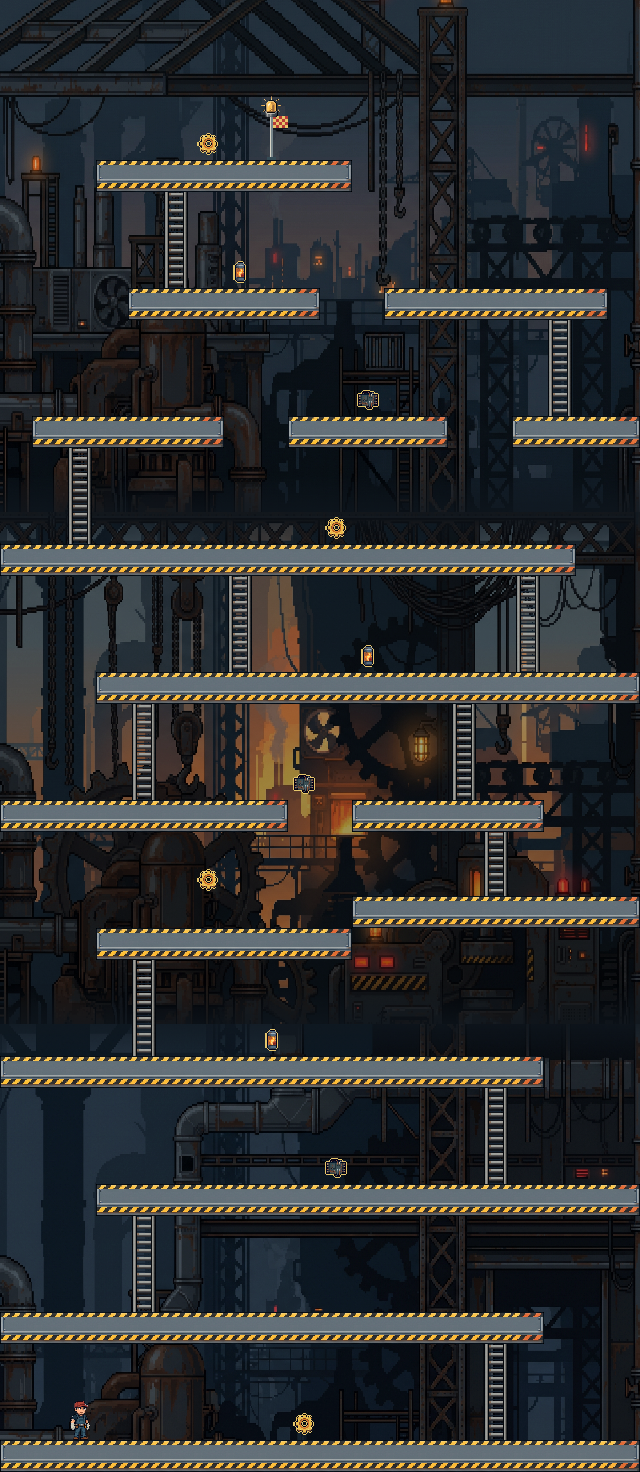
\includegraphics[width=\linewidth]{figs/GameLevel_Full.png}
\captionof{figure}{Nivel completo (zonas 1, 2 y 3 de abajo arriba).}\label{fig:nivel}
\end{minipage}

\section{Comportamiento autónomo (barriles)}
Cada barril es un agente con una máquina de estados: \emph{Aparece} $\rightarrow$ \emph{Rueda}
$\rightarrow$ \emph{Cae} $\rightarrow$ \emph{Rueda} (en sentido contrario) $\rightarrow \dots$
$\rightarrow$ \emph{Destruido}. Mientras rueda comprueba si tiene suelo bajo el centro (si no, cae) y
si hay una pared delante (si la hay, termina su recorrido). El generador de cada zona decide cuándo
lanzar el siguiente barril según la velocidad y la frecuencia configuradas para esa zona, de modo que
la presión aumenta al subir.

\section{Condición de término}
\begin{itemize}
\item \textbf{Victoria:} tocar la baliza de la cima. Se detiene el tiempo, se paran los barriles y se
muestra la puntuación final con los botones \emph{Reiniciar} y \emph{Menú}.
\item \textbf{Derrota:} perder las tres vidas. Se muestra \emph{Game Over} con la puntuación obtenida y
las mismas opciones.
\item \textbf{Salir:} en cualquier momento desde la pausa (\emph{Menú}) o desde el menú principal (\emph{Salir}).
\end{itemize}

\section{Bucle principal y progresión}
El ciclo de juego que se repite en cada piso es: \textbf{observar} el patrón de los barriles
$\rightarrow$ \textbf{decidir} (esperar, saltar, pisar o desviarse por un coleccionable) $\rightarrow$
\textbf{moverse} hasta la escalera $\rightarrow$ \textbf{subir} al piso siguiente. Al cambiar de zona
aparece un aviso (\emph{``ZONA 2''}), se suma el bonus y los barriles se vuelven más rápidos y
frecuentes. La tensión crece así de forma natural con la altura, hasta el último piso, donde la baliza
queda a la vista y el jugador debe cruzar vigas estrechas con huecos.

\begin{figure}[h]
\centering
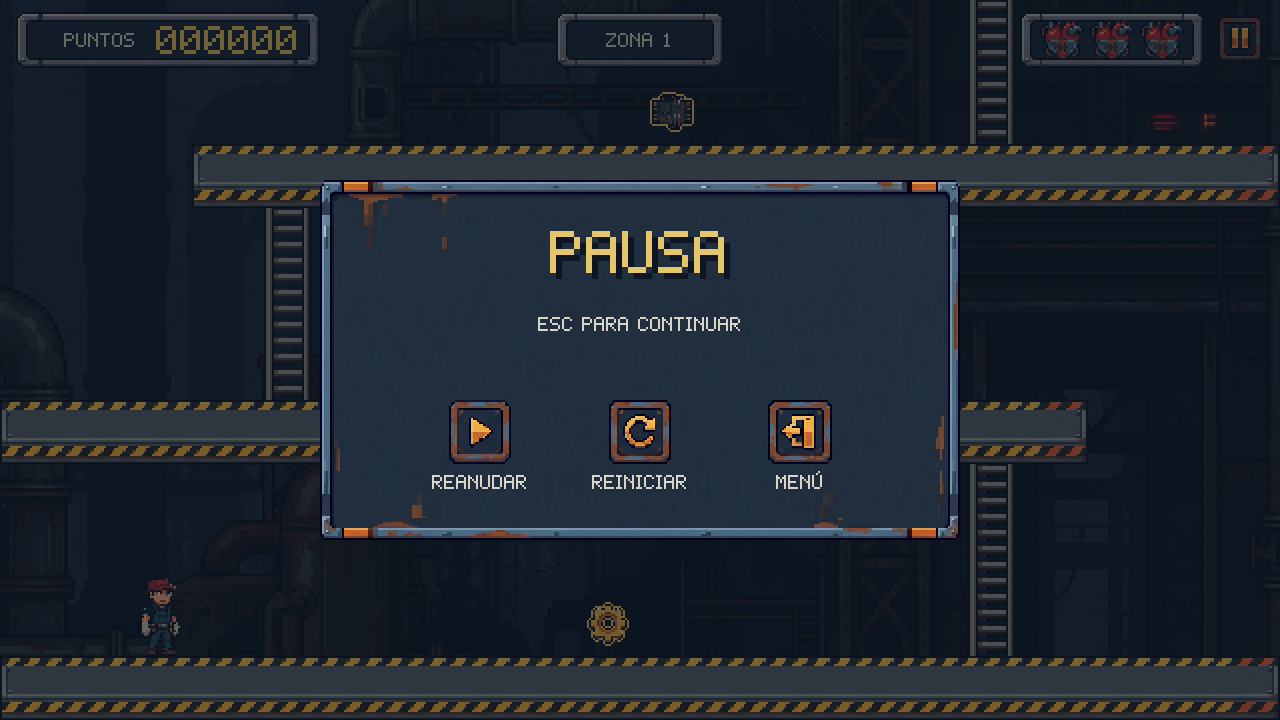
\includegraphics[width=0.32\linewidth]{figs/UI_PausePanel.png}\hfill
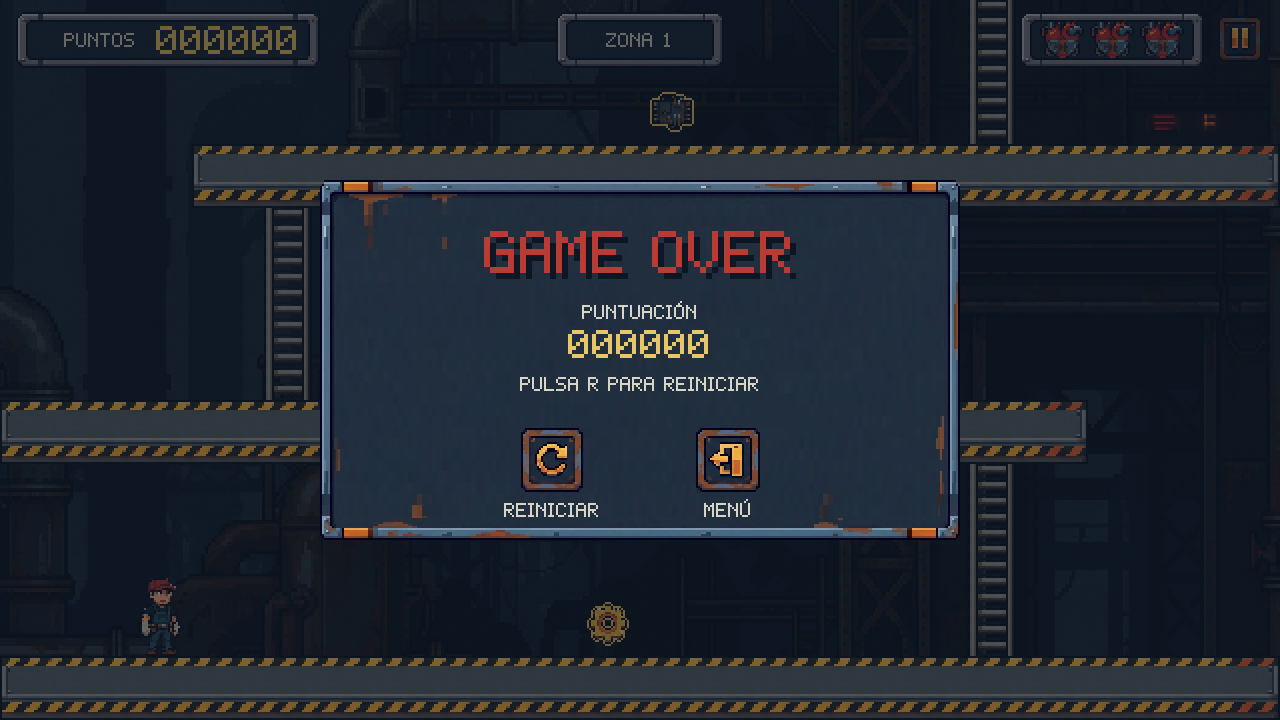
\includegraphics[width=0.32\linewidth]{figs/UI_GameOverPanel.png}\hfill
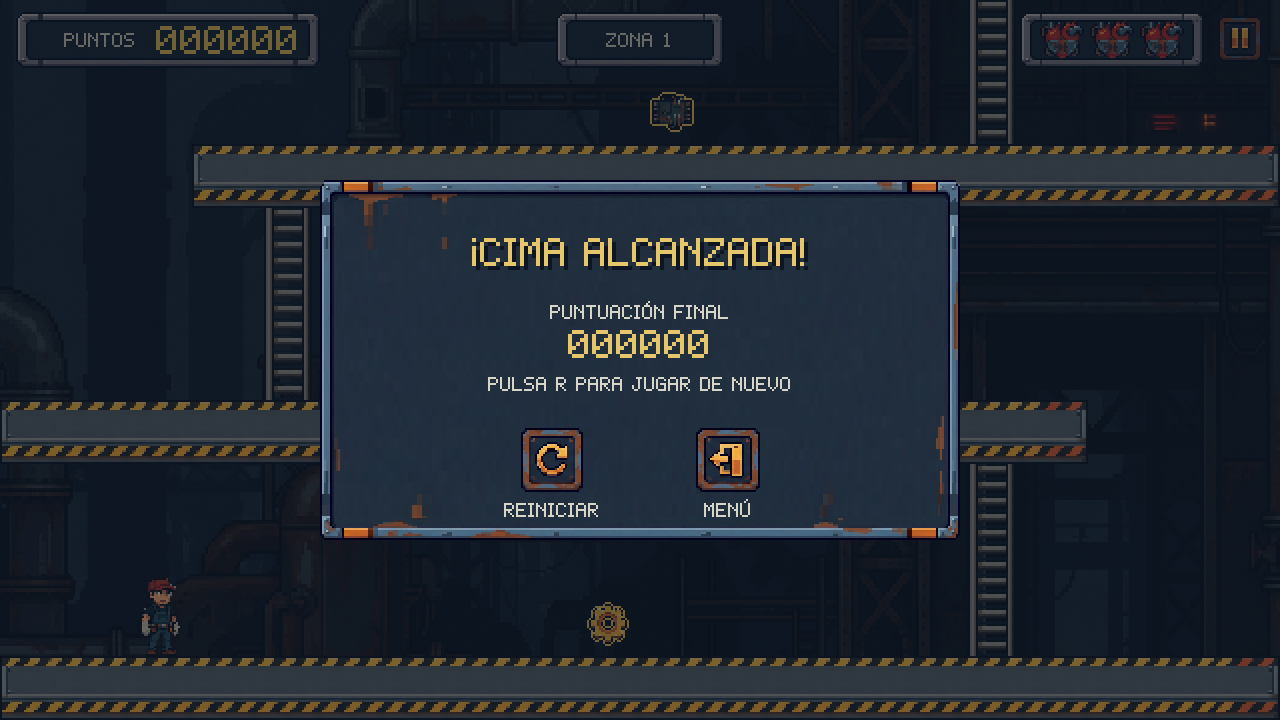
\includegraphics[width=0.32\linewidth]{figs/UI_VictoryPanel.png}
\caption{Paneles de Pausa, Game Over y Victoria, cada uno con su puntuación y botones de reinicio y menú.}
\end{figure}

\section{Estética, audio y recursos}
Pixel art a 640$\times$360 (escalado $\times$3 exacto en 1080p) con una paleta industrial de azules oscuros,
óxido y amarillo de advertencia. Música en bucle distinta para menú y partida, y efectos de sonido para
salto, aterrizaje, pisotón, recogida, daño, zona completada, pausa, botones, victoria y derrota.
Los sprites, el tileset, los fondos y la interfaz fueron creados por la autora con la IA generativa
Gemini de Google y procesados en Unity; la música y los efectos de sonido provienen de Pixabay
(pixabay.com), con su licencia de contenido gratuito. La fuente pixel de la interfaz se generó desde código.
El detalle técnico de cada componente está en el reporte técnico.

\end{document}
